\newif\ifvimbug
\vimbugfalse

\ifvimbug
\begin{document}
\fi

\exercise{Density Estimation}
In this exercise, you will use the datasets \texttt{densEstClass1.txt} 
and \texttt{densEstClass2.txt}. The datasets contain 2D data belonging
to two classes, $C_1$ and $C_2$.

\begin{questions}

%----------------------------------------------

\begin{question}{Gaussian Maximization Likelihood Estimate}{10}
Derive the ML estimate for the mean and covariance of the \textbf{multivariate} Gaussian distribution. Start your derivations with the function you optimize. Assume that you can collect i.i.d data. (Hint: you can find many matrix identities on the Matrix Cookbook and at \url{http://en.wikipedia.org/wiki/Matrix_calculus}.)

\begin{answer}

%First we take a look at the optimization function:\\
\begin{align*}
L(X | \theta ) &= max \log p(X|\theta ) \\
&= \log \prod_{i=1}^{N} p(x_i|\theta ) \\
&= \sum_{i=1}^{N} \log p(x_i|\theta ) \\
&= \sum_{i=1}^{N} \log ( (2\pi )^{-\frac{K}{2}} |\Sigma |^{-\frac{1}{2}} \exp (-\frac{1}{2} (x_i-\mu )^{T} \Sigma^{-1}(x_i-\mu ))) \\
&= \sum_{i=1}^{N} ( \log ((2\pi )^{-\frac{K}{2}}\Sigma^{-\frac{1}{2}})-\frac{1}{2} (x_i-\mu )^T \Sigma^{-1}(x_i-\mu) ) \\
&= -\frac{N K}{2} \log (2\pi )-\frac{N}{2} \log |\Sigma |-\frac{1}{2}\sum_{i=1}^{N}(x_i-\mu )^T \Sigma^{-1}(x_i-\mu )\\
\end{align*}

1. In order to compute the ML estimate for the mean we take the derivative for $\mu $:
\begin{align*}
\frac{\delta L}{\delta \mu} &= \frac{\delta(-\frac{1}{2}\sum_{i=1}^{N}(x_i-\mu )^T \Sigma^{-1} (x_i-\mu ))}{\delta \mu} \\
&= -\frac{1}{2} \sum_{i=1}^{N}(-(x_i-\mu )^T \Sigma^{-1}-(x_i-\mu )^T \Sigma^{-1}) \\
&= \sum_{i=1}^{N}(x_i-\mu )^T\Sigma^{-1}
\end{align*}
Setting it to zero gives us the following formular for the mean:
\begin{align*}
0 &= \sum_{i=1}^{N}(x_i-\mu )^T\Sigma^{-1} \\
\Leftrightarrow \quad 0 &= \sum_{i=1}^{N}(x_i-\mu ) \\
\Leftrightarrow \quad 0 &= \sum_{i=1}^{N}x_i^T-N\mu^T \\
\Leftrightarrow \quad \mu &= \frac{1}{N}\sum_{i=1}^{N}x_i 
\end{align*}

2. In order to compute the ML estimate for the covariance we take the derivative for $\Sigma$:
\begin{align*}
\frac{\delta L}{\delta \Sigma} &= \frac{\delta (-\frac{N}{2} \log |\Sigma |)}{\delta \Sigma} - \frac{1}{2} \frac{\delta (\sum_{i=1}^{N}(x_i-\mu )^T \Sigma^{-1}(x_i-\mu ))}{\delta \Sigma}\\
&= -\frac{N|\Sigma |\Sigma^{-1}}{2|\Sigma |}-\frac{1}{2} \frac{\sum_{i=1}^{N} \delta (Tr(x_i-\mu )^T \Sigma^{-1}(x_i-\mu ))}{\delta \Sigma} \\
&= -\frac{N}{2} \Sigma^{-1} - \frac{1}{2} \frac{\sum_{i=1}^{N} \delta ( Tr\Sigma^{-1}(x_i-\mu )(x_i-\mu )^T)}{\delta \Sigma} \\
&= -\frac{N}{2} \Sigma^{-1} + \frac{1}{2} \sum_{i=1}^{N} \Sigma^{-1} (x_i-\mu )(x_i-\mu )^T \Sigma^{-1} \\
&= -\frac{N}{2} + \frac{1}{2} \sum_{i=1}^{N} \Sigma^{-1} (x_i-\mu )(x_i-\mu )^T
\end{align*}
Then we set the derivative to zero:
\begin{align*}
0 &= \frac{\delta L}{\delta \Sigma} \\
\Leftrightarrow \quad 0 &= -\frac{N}{2} + \frac{1}{2} \sum_{i=1}^{N} \Sigma^{-1} (x_i-\mu )(x_i-\mu )^T \\
\Leftrightarrow \quad \frac{N}{2} &= \frac{1}{2} \Sigma^{-1} \sum_{i=1}^{N} (x_i-\mu )(x_i-\mu )^T \\
\Leftrightarrow \quad N &= \Sigma^{-1} \sum_{i=1}^{N} (x_i-\mu )(x_i-\mu )^T \\
\Leftrightarrow \quad \Sigma &= \frac{1}{N} \sum_{i=1}^{N} (x_i-\mu )(x_i-\mu )^T \\
\end{align*}

\end{answer}
\end{question}


%----------------------------------------------

\begin{question}{Prior Probabilities}{2}
Compute the prior probability of each class from the dataset. 

\begin{answer}
Dataset 1 has 239 elements, dataset 2 has 761 elements, resulting in 1000 elements total. Therefore:\\
$p(C_1) = \frac{239}{1000}=0.239$, $p(C_2) = \frac{761}{1000}=0.761$
\end{answer}

\end{question}


%----------------------------------------------

\begin{question}{Biased ML Estimate}{5}
Define the bias of an estimator and write how we can compute it.
Then calculate the biased and unbiased estimates of the conditional distribution $p(x|C_i)$, assuming that each class can be modeled with a Gaussian distribution. Which parameters have to be calculated?
Show the final result and attach a snippet of your code.
Do not use existing functions, but rather implement the computations by yourself!

\begin{answer}
The bias of an estimator is the failure/difference between the estimated value and the true value. The formular is:
\[
	bias(\Theta )=E_x(\Theta (X)-\Theta )
\]

Our results for classes 1 and 2 are:
\begin{align*}
\mu_1 &= \begin{pmatrix} 
-0.70386868 \\
-0.81004153 \\
\end{pmatrix} \\
\Sigma_{1, biased} &= \begin{pmatrix}
9.01953453 & 2.67288083 \\
2.67288083& 3.59635114 \\
\end{pmatrix} \\
\Sigma_{1, unbiased} &= \begin{pmatrix}
8.98195314 & 2.66174383 \\
2.66174383 & 3.58136635 \\
\end{pmatrix} \\ \\
\mu_2 &= \begin{pmatrix} 
3.98011241 \\
3.97915479 \\
\end{pmatrix} \\
\Sigma_{2, biased} &= \begin{pmatrix}
4.17540885 & 0.02761059 \\
0.02761059 & 2.75299057 \\
\end{pmatrix} \\
\Sigma_{2, unbiased} &= \begin{pmatrix}
4.16992931 & 0.02757436 \\
0.02757436 & 2.74937772 \\
\end{pmatrix}
\end{align*}
Our python code looks as following:\\
\lstinputlisting[language=Python, firstline = 1]{dataSets/python_2_2/python-code.py}
\end{answer}

\end{question}


%----------------------------------------------

\begin{question}{Class Density}{5}
Using the unbiased estimates from the previous question, fit a Gaussian distribution to the data of each class. Generate a single plot showing the data points and the probability densities of each class.
(Hint: use the contour function for plotting the Gaussians.) 

\begin{answer}
\centering 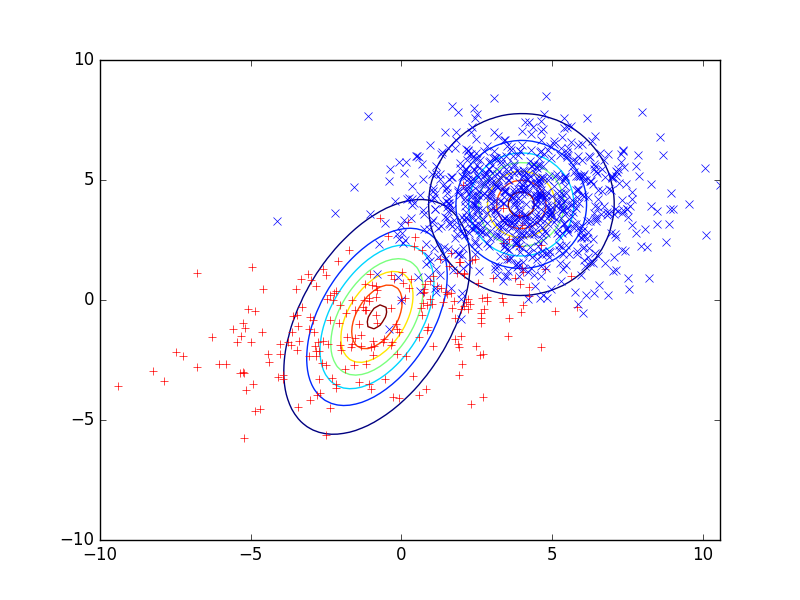
\includegraphics[width=1.0\linewidth]{dataSets/2-2-d}\label{fig:gaussians}
\end{answer}

\end{question}

%----------------------------------------------

\begin{question}{Posterior}{8}
In a single graph, plot the posterior distribution of each class $p(C_i|x)$ 
and show the decision boundary. For convenience, show the probabilities
in the log domain.

\begin{answer}
\centering 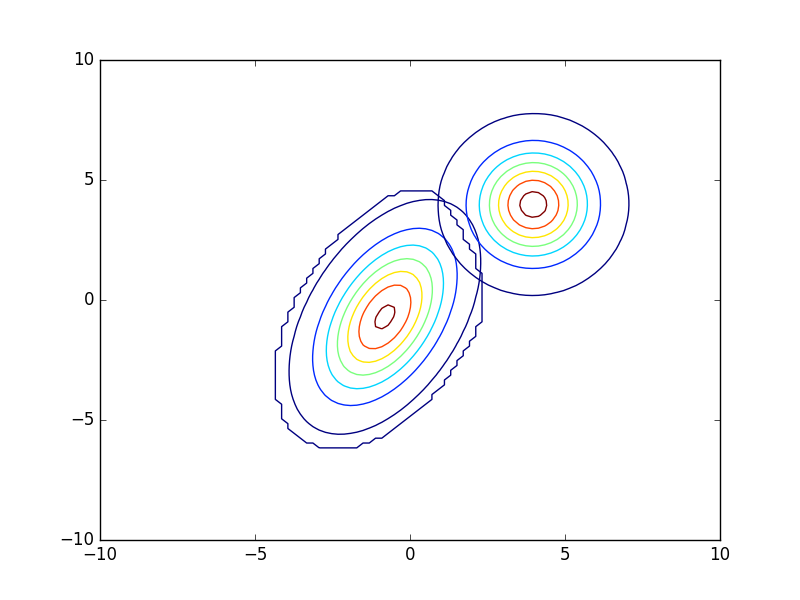
\includegraphics[width=1.0\linewidth]{dataSets/2-2-e}\label{fig:decisionboundary} \\
Note: Sorry for the unclear colering. The \emph{jagged} blue line is the decision boundary.
\end{answer}

\end{question}

%----------------------------------------------

\begin{question}{Bayesian Estimation}{15}{bonus}
State the generic case of a Bayesian treatment of the parameters $\theta$ used to model the data, .i.e., $p(\vec X \middle | \theta )$. 
Which are the advantages of being Bayesian? 
\\ Derive the estimate of the mean, assuming that the model is a Gaussian distribution with a fixed variance. (Hint: work approximately, complete the square.)


\begin{answer}
The generic case of the Bayesian treatment with parameters $\theta$ looks as follows:
\[
	p(x|X)=\int p(x|\theta )p(\theta | X)d\theta
\]
Advantages of being Bayesian is that we can average over all parameters instead of fixing to a limited subset. It is also possible to consider priors to the parameters. The estimated probability indicates how uncertain our predictions of our model are. In order to derive the estimate of the mean we procede as follows. \\
\\
We assume the prior distribution of the mean to be given as $\mu \approx N(\mu |\mu_0, \sigma_0$. Then we can estimate:

\begin{align*}
p(\mu|X) &= \frac{p(X|\mu)p(\mu)}{p(X)} \\
&= N(\mu|\mu_N,\sigma_n)
\end{align*}
This is a gaussian distribution and we can exploit the following formula for the mean:
\begin{align*}
\sigma_N^2=\frac{\sigma^2\sigma_0^2}{\sigma^2+N\sigma_0^2}
\end{align*}
Therefore the mean can be transformed as, where $\mu'$ is the sampled mean with $\mu'=\frac{1}{N}\sum_{i=1}^{N}x_i$.
\begin{align*}
\mu_N &= \frac{1}{\sigma^2+N\sigma_0^2}(\sigma_0^2 \sum_{i=1}^{N}x_i+\sigma^2+\mu_0) \\
&= \frac{\sigma_0^2N\mu' + \sigma^2\mu_0}{\sigma^2+N\sigma_0^2}
\end{align*}


\end{answer}

\end{question}

\end{questions}
